
\section{Testing Services}
\label{sec:testing-debugging}

Within the increasing demand for software development as a service,
\textit{software testing as a service} has seen significant growth and adoption
in its own right.  Software testing as a service is a multi-billion dollar (annually) 
market, growing at about 20\% per year. Testing services as an area is a microcosm
of the entire services landscape.

%In fact, according to a 2006 survey,\footnote{\scriptsize
%  \url{http://www.drdobbs.com/architecture-and-design/cheapers-not-always-better/184415486?requestid=247829}}
%software testing was the second largest outsourced software-engineering activity
%after coding: 81\% of the 200 industrial practitioners, who participated in the
%survey, stated that they outsource software testing. Given this trend, services
%companies now routinely offer services that focus exclusively on testing
%activities, 

%% The engagement modes can vary: staff augmentation, core/flex, managed service
%% (fixed capacity, outcome based). But perhaps this needs to be mentioned earlier
%% as these modes are not particular to testing services.

\begin{figure}[t]
\centering
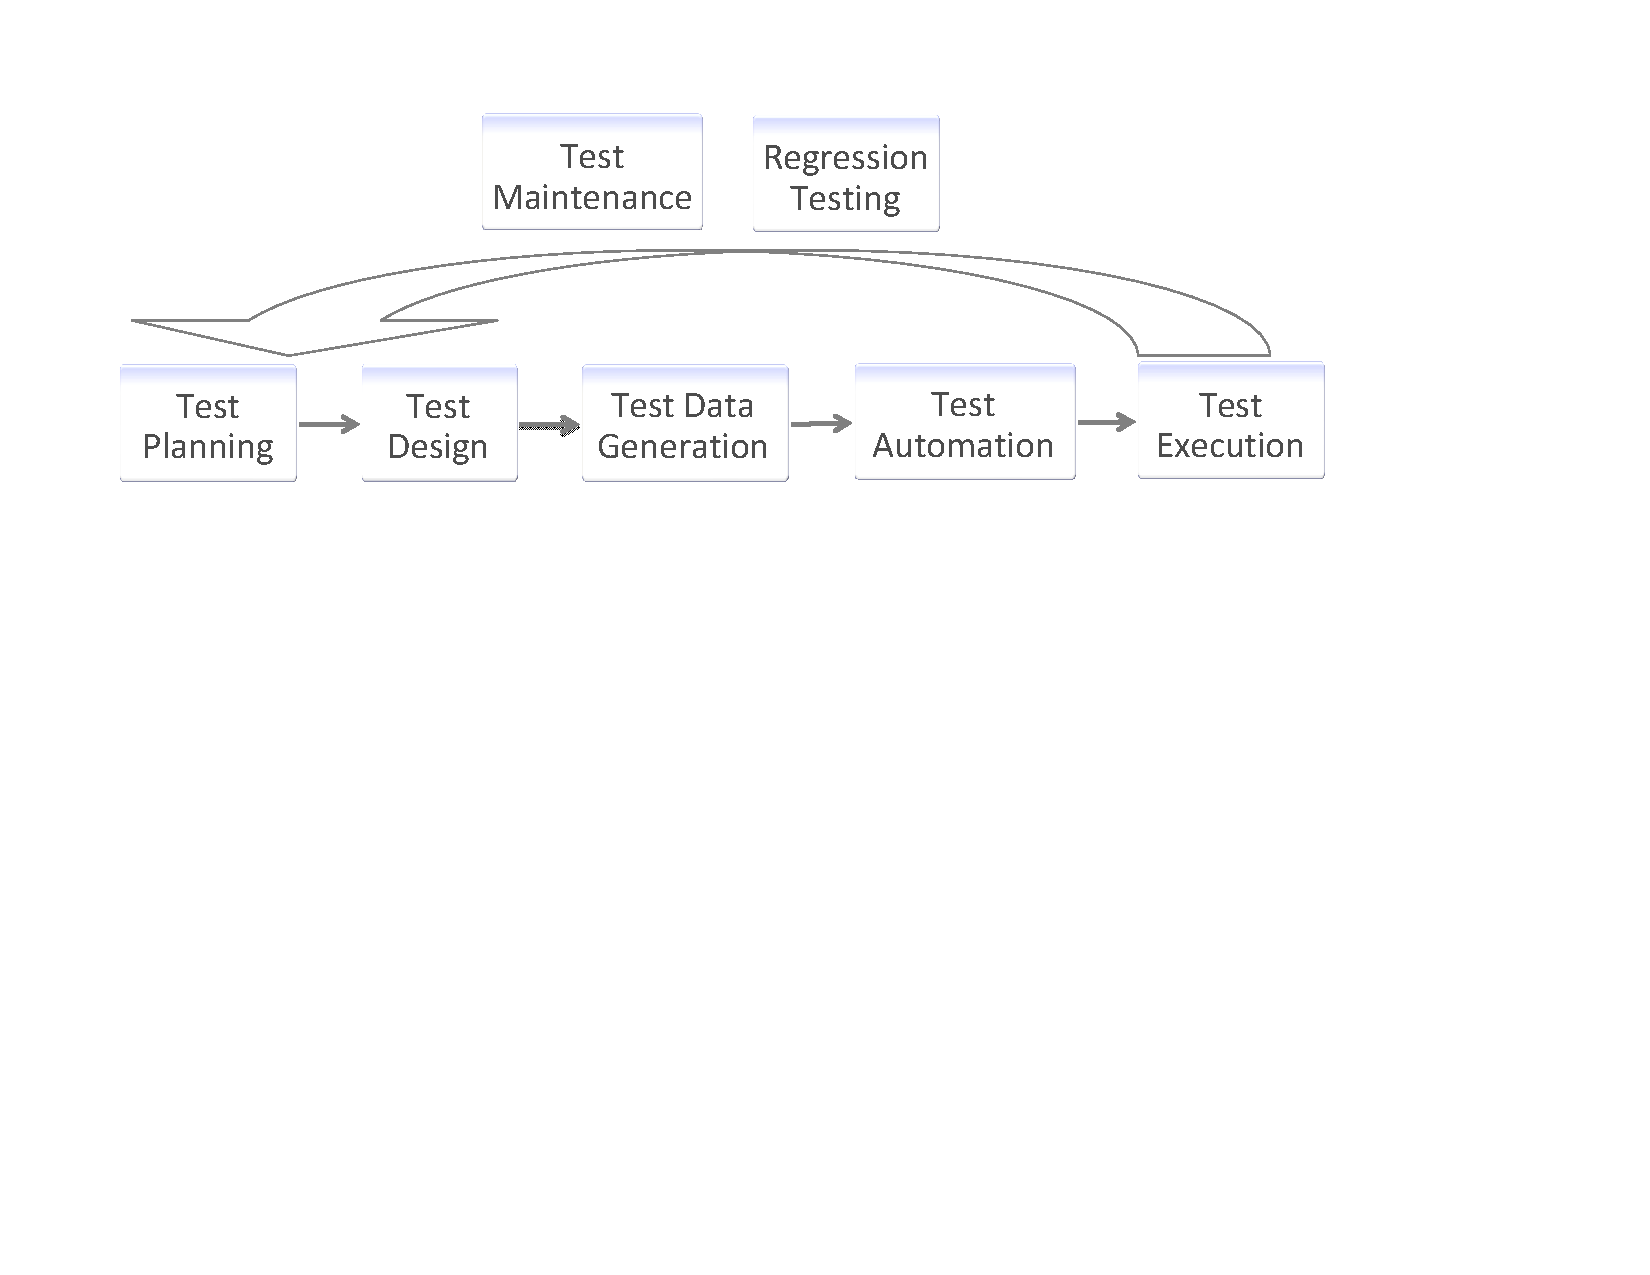
\includegraphics[width=\columnwidth, clip, trim = 22mm 133mm 65mm
  17mm]{figs/testing-activities.pdf}
\vspace*{-15pt}
\caption{Typical testing activities performed in delivery of testing services.}
\vspace*{-10pt}
\label{fig:testing-activities}
\end{figure}

The nature of the activities performed in a testing-services engagement can vary
from client to client. The scope of work can include any of test planning, test design,
test-data creation, test automation, test execution, and test maintenance. 
Figure~\ref{fig:testing-activities} presents an overview of
the commonly performed activities in testing services. 
A particular engagement might involve any subset of these activities; for example,
tesing for a client might involve only test execution, with the other
activities done by the client or by other vendors.  
%% The nature of
%% the test cases can also vary from functional tests to tests that focus on
%% validating non-functional system properties, such as performance and security.

%% The activities shown in Figure~\ref{fig:testing-activities}, of course, pertain
%% to testing in general (whether performed in-house or in an outsourced manner),
%% but there are factors that can add unique challenges in the setting of testing
%% services.  

Although software testing appears to be full of opportunities for automated tools,
for a variety of reasons, testing services remains largely a labor-intensive
business.  For example, manual testing of GUI-based applications is surprisingly
common, and testers routinely make up test data without methodical analysis.

Here are some of the reasons testing services is labor intensive.  First is that
the automated techniques available today do not necessarily hold up to enterprise
applications, which include a heteregenous mix of languages and technologies, and
for which requirements are written in prose by business analysts.
Second, none of the techniques that require source code analysis or inspection
are typically applicable because the vendor offering testing services is given
only ``black box'' access to the system under test.  Third, deliverables of testing
activity must be shown rather quickly (because revenues for the vendor are
tied to deliverables), and a long investment in time and money that
is needed in deployment of a tool is rarely tolerated either by the vendor or the
client.  A related reason is that the supply of labor that can deliver testing services 
has hitherto been plentiful and affordable, reducing the economic motivation to invest 
in tools.

The only ``testing'' tools that are routine in use in testing services are test management 
and reporting tools that help keep track of which tests have been run (often manually) along with
their outcomes.

However, given the growth in testing services, it is inevitable that it needs to move from
a labor intensive business to an assets and tools-based business.  Therefore, 
research in this area is about automated tools so that 
testing can be carried out at lower cost and with consistent quality.  
Implicit in the abovementioned reasons is that the proposed solutions should be 
quick to deploy, low cost, and accessible to a large labor pool.

%%For instance, many of these activities can require specific skills in
%%testing techniques/tools or coding expertise, which the average testing
%%practitioner involved in service delivery may not possess. Second, some of the
%%activities may need to be carried out in strict time-bound cycles (governed by
%%service-level agreements) and in client-controlled test environments. Finally,
%%the myriad of technologies that must be accommodated in the contexts of the IT
%%systems of different clients adds another layer of complexity for service
%%companies.

%%Thus, in the setting of testing services, with its unique characteristics and
%%challenges, manual test creation, execution, and maintenance is still done quite
%%often.  The main goal of introducing innovation in this setting is to bring
%%automation and rigor to the testing tasks that are performed manually, sometimes
%%in an ad-hoc manner, and are prone to human lapses.

%%The testing research community has seen a long line of research (running into a
%%few decades) developing automated techniques for a variety of testing
%%problems---such as test-adequacy assessment, test-input generation, regression
%%test selection, test augmentation, test prioritization, and test
%%minimization---for imperative and object-oriented programs, and applicable to
%%different types of systems (\eg component-based systems and web
%%applications). For instance, there exists a large body of techniques for
%%automated test-input generation (\eg ~\cite{Artzi:2011, Boyapati:2002, cadar08,
%%  Clarke:1976, Ferguson:1996, godefroid05, Gross:2012, Harman:2010, king76jul,
%%  korel90aug, Pacheco:2007, sen05, thummalapenta:2011, Tillmann:2005,
%%  visser04}).  But, many of the techniques are inapplicable, or at least there
%%are significant challenges in applying them, in the context of testing
%%services. As already mentioned, most enterprise applications include a mix of
%%languages and technologies; thus, the automated techniques must deal with this
%%complexity. Second, in testing services, the vendor often does not have access
%%to the source code of the applications under test; thus, program-analysis-based
%%techniques would be inapplicable in these cases. Third, many automated
%%techniques---\eg much of the research on test-input generation---focus on unit
%%testing, which is not in the scope of work in testing services.

In the rest of this section, we discuss the testing activities shown in
Figure~\ref{fig:testing-activities}. For each activity, we present a sample of
relevant existing research and identify important unsolved (or partially solved)
problems for which the development of new automated techniques would make
valuable research contributions.

\subsection{Test Planning and Optimization}
\label{sec:test-planning}

Test planning involves tasks such as establishing the test process or strategy,
allocating resources, estimating cost and schedule, defining test-environment
requirements, identifying test targets, determining risk profiles for targets,
projecting defects and test numbers for each target, etc.  Test planning can be
done at multiple levels---such as macro planning at the start of a project which
evolves into micro planning as the project proceeds---and the test plan needs to
be continuously refined during the course of a project as more accurate
information becomes available.

\subsubsection*{Research topic: ROI on Testing}

Test planning is intended not only to guide all downstream testing activities,
including test design, test execution, test-data and test-environment
provisioning, test reporting, etc., it should also answer key business
questions, such as~\cite{Kagan:NextGenTesting}

\begin{itemize}
\denseitems

%%\item How do we determine the quality of our testing effort?

\item Are we getting our money's worth out of testing?

\item Are we doing too much or too little testing?

\item Will an increased testing investment drive further improvement in quality?

%%\item Our testing budget was cut---what testing should we eliminate what will be
%%  its impact on product quality?

\end{itemize}

It has long been believed that more the testing, less the likelihood of defects escaping
to the field, and yet there is a point of diminishing return at which it is no longer 
cost effective to invest in testing.  However, this judgment is
made mostly on intuition.  Little is available to managers by way of quantititive techniques
to balance the cost and benefit of continued testing.  Therefore, one of the
research problems is to mine historical project data across a number of projects
to formulate techniques for balancing the cost of testing with the return that it 
provides in terms of risk reduction.  Li and Boehm (http://dl.acm.org/citation.cfm?id=2486061) 
have recently presented an approach to prioritize tests based on their business value.

%One of the challenges in test planning is standardizing and automating it, using
%data intelligence and forecasting. The availability of appropriate data is
%central to accurate forecasting and construction of prediction models (\eg for
%defect prediction). Although in a project, such data may be scarce initially, in
%the context of testing services, the vendor has the opportunity to mine and
%leverage data from hundreds of client projects to build benchmark data that can
%improve the accuracy of even the initial estimates in a project. This is another
%instance of the problem of capturing and leveraging organizational knowledge,
%across multiple client engagements, discussed in Section~\ref{sec:km}. In the
%context of test planning, we see further opportunities for research
%contributions in the types of data to be mined, anonymized, cataloged, linked,
%and organized for use in building accurate prediction models for testing-related
%activities.

\subsubsection*{Research topic: Efficient Test Optimization}

In a testing-service engagement, a vendor can inherit existing test cases,
possibly designed by another vendor, for the applications under test. In fact,
in large testing-services engagements, the number of such test cases can easily
run into tens of thousands (sometimes even exceeding a couple of hundred
thousand).  To make matters worse, often, the test cases are captured in natural
language, stored in unstructured and varying formats (\eg in plain-text
documents or spreadsheets), and contain redundancies. 
%Thus, the vendor testing
%teams face the daunting task of taking stock of the available test cases,
%understanding them, and optimizing them.

Tools for extracting relevant information about test cases (\eg test name, test
steps, test prerequisites, expected outcome) from the diverse formats of
natural-language descriptions, and tools for clustering test cases (based on the
natural-language descriptions of tests) would be extremely valuable in assisting
testers in efficiently getting a good handle on a large corpora of unfamiliar
test cases. 
%Techniques from natural-language-processing and machine-learning
%communities can be profitably leveraged toward solving these problems.

Since it is generally infeasible to run such a large number of tests in each
regression cycle, testers must decide which tests to run.  And despite the
size, a test suite may not give a balanced coverage of the application.
Thus, techniques are needed to select test scenarios systematically.  

One such technique---used extensively at IBM---is combinatorial test design 
(CTD)~\cite{Cohen:1996, Cohen:1997, Cohen:2003}.
With CTD, first an application's behavior is modeled in terms of key attributes,
and points of variability of each attribute are determined. Then, an algorithm
systematically generates combinations of attribute-values that should be exercised.
CTD manages combinatorial explosion in a principled way, e.g. by testing only
every 2-way combinations of attributes-values.  However, use of CTD requires high domain expertise
and modeling skill, which is an inhibitor to its broad adoption.  Effective tool 
support for simplifying modelconstruction~\cite{Segall:2012a}, iteratively refining
models~\cite{Segall:2012b}, and debugging models~\cite{Farchi:2013} is an active
area of research, with scope for more contributions, \eg in supporting model
maintenance and evolution.  
%%Assuming that accurate CTD models can be created for a client system, a
Another challenging unsolved problem is how to map the output of CTD 
%(\ie a $k$-way covering array) 
to the existing test cases. This is a very tedious task, almost
completely manually performed, for which tool support would be very valuable in
practice.

%Another task that testers have to perform is optimizing large test suites by
%removing redundant tests while ensuring good test diversity and
%coverage.\footnote{\small Test optimization can also be addressed at the
%  test-execution level, which we discuss in Section~\ref{sec:test-maintenance};
%  in this section, we focus on design-level optimization.} Combinatorial test
%design (CTD)~\cite{Cohen:1996, Cohen:1997, Cohen:2003} is a useful technique for
%performing such optimization that has been rigorously researched. Applying CTD
%in the context of testing services, with the available skill level and the
%effort that goes in creating CTD models for an unfamiliar system---by
%identifying attributes and values (or points of variability), and
%restrictions---can be challenging. Effective tool support for simplifying model
%construction~\cite{Segall:2012a}, iteratively refining
%models~\cite{Segall:2012b}, and debugging models~\cite{Farchi:2013} is an active
%area of research, with scope for more contributions, \eg in supporting model
%maintenance and evolution.



\subsection{Test Data Generation}
\label{sec:test-data}

\subsection{Test Data Generation}

Enterprise applications are typically database-oriented, in that they make queries over databases and the program flow depends on the data retrieved as a result of a query.  In order to test whether the application satisfies its requirements, sufficient amount of test data must be made available in the database. Consider, for example, a banking application, in which one of the requirement to exercise is that if a customer makes a certain fixed deposit, and the person is a senior citizen, and also holds a checking account in the bank, then an addition 0.25\% is paid as interest. To test that this situation is handled correctly in the application, there should exist a customer in the database such that his or her age qualifies the person as senior citizen and the person also has a checking account. Notice that typically, customer data and account data would be maintained in separate database tables. Typically business requirements are complex, and there need to be specific entries in multiple tables for a scenario to work out.

When a client gives a testing contract, the client may expect the service provider to exercise all the business rules, but may not give enough sample data in the database to be able to exercise these rules.  It then becomes the responsibility of the service provider to figure out the requisite test data to be present in the pertinent tables.

Randomly generated test data  cannot be expected to suffice for enterprise applications with complex rules. Also, systematic test generation approaches based on program analysis cannot be expected to tackle enterprise application, which use a mix of multiple language and database technologies in their implementation. The database community has done some work in creating test data for SQL queries, and that may be relevant; however, as mentioned before, enterprise applications are implemented with a mix of technologies.

We see a big opportunity for research contributions in this subarea. How to take a specification of the application as testing criteria, and automatically populate database that would enable various scenarios that fulfill the test criteria to be exercised.


\subsection{Test Automation}
\label{sec:test-automation}

The functional test cases for enterprise applications are often stated
informally in natural language. These tests are known as \textit{manual test
  cases}, which consist of a sequence of steps, intended for execution by a
human on the application user interface (UI).  Test automation is the activity
of converting these test cases into test scripts or programs that perform the
test steps mechanically. After creation, the automated test scripts can be
executed in regression cycles without any human intervention. For example,
Figure~\ref{fig:sample-test-case} shows a manual test case written in plain
English (left) and the corresponding tool-agnostic automated test script
(right). Typically, some amount of metadata necessary for locating the UI
elements is also stored in the test scripts.

\begin{figure}[t]
\centering
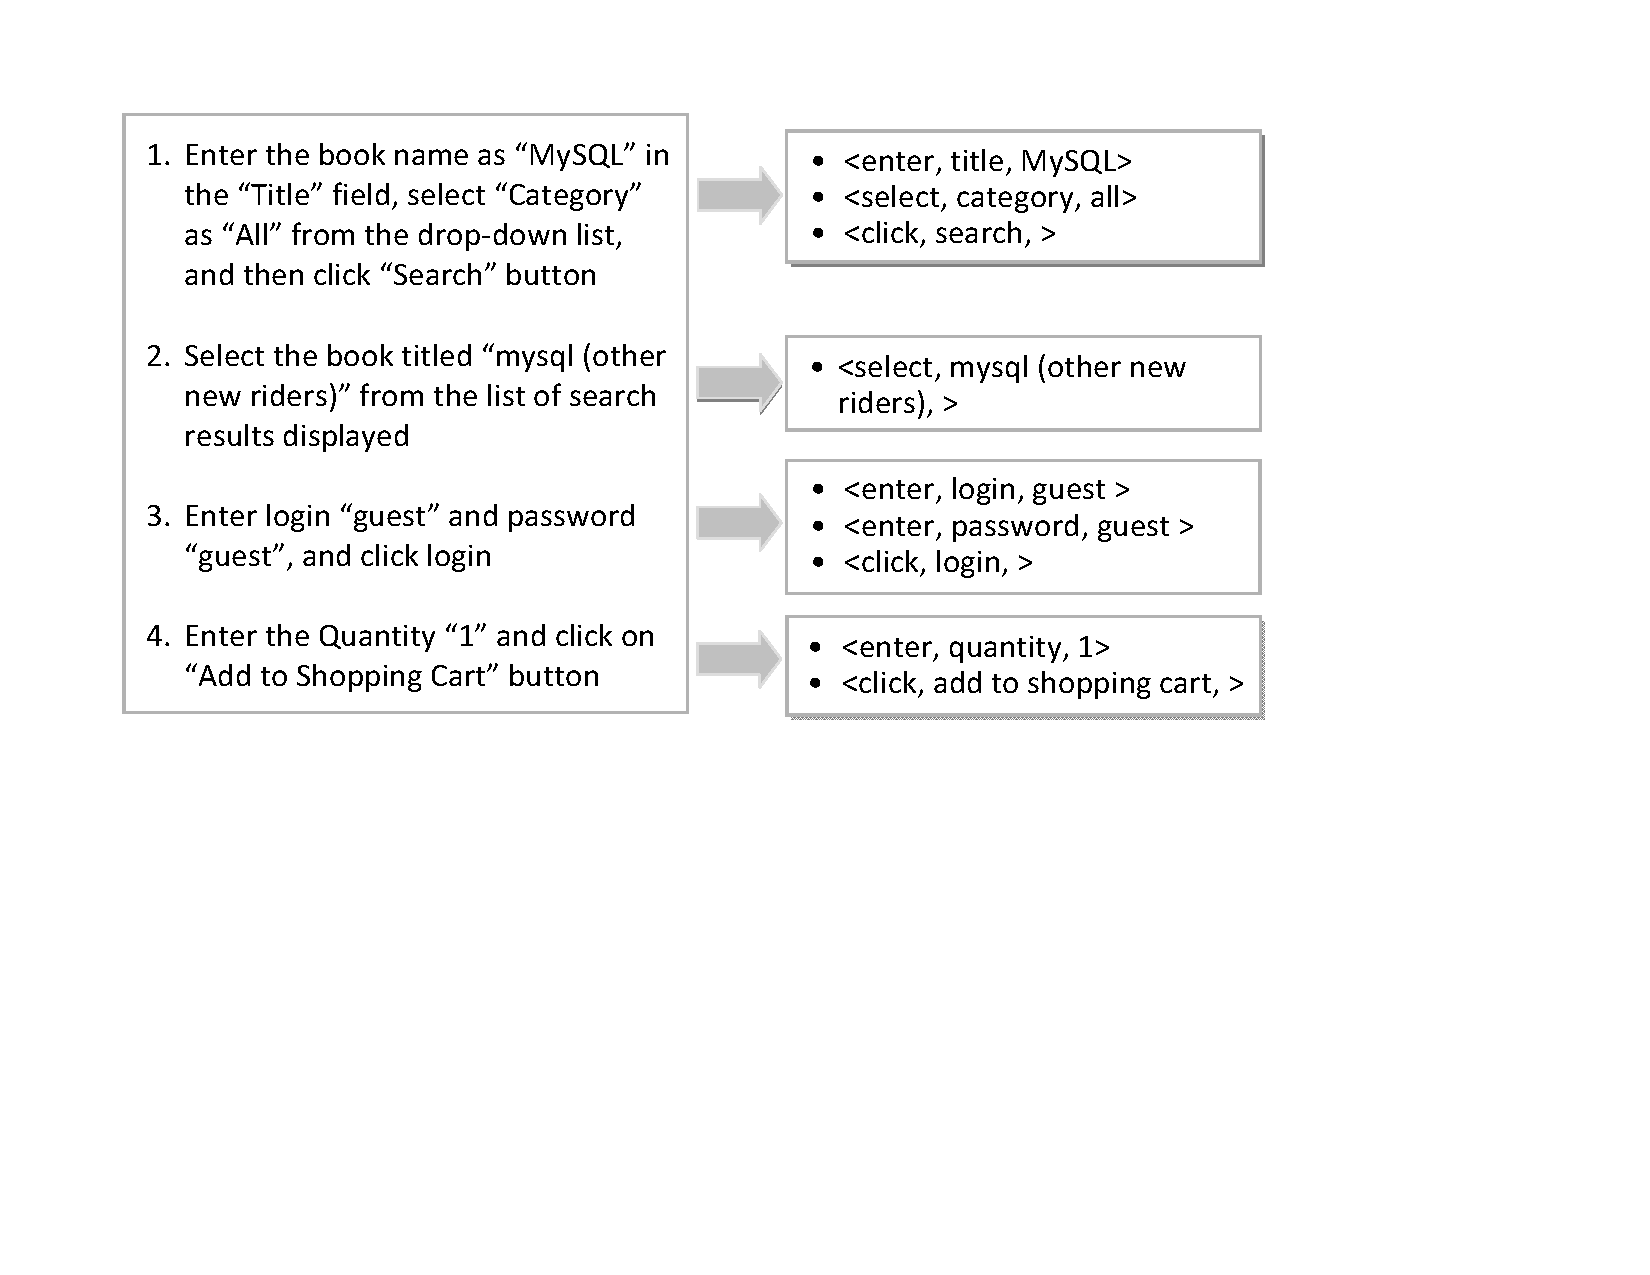
\includegraphics[width=\columnwidth, clip, trim = 21mm 93mm 65mm
  18mm]{figs/sample-test-case.pdf}
\vspace*{-15pt}
\caption{Sample manual test case and tool-agnostic script representation.}
\vspace*{-10pt}
\label{fig:sample-test-case}
\end{figure}

Although test automation is desirable (\eg for efficient and predictable test
executions) and sometimes necessary (\eg to meet time-constrained regression
schedules), creating \textit{robust} test scripts that can be used repeatedly in
regression cycles is expensive. In essence, creating such scripts is
time-consuming, involving a significant amount of coding, and requires expertise
in test automation tools (\eg \cite{hpqtp,ibmrft,selenium}). In the context of
testing services, this poses the unique challenge: how can change-resilient test
scripts be created efficiently by delivery personnel who may not possess good
programming skills or deep tool knowledge? 

%% Moreover, test automation involves not only the one-time cost of creating the
%% scripts, but also a recurring cost of maintaining the scripts in response to
%% application changes and changes in the execution environment.

\subsubsection*{Research topic: Creating Robust Test Scripts}

The core problem that needs to be addressed in creating robust test scripts is
how to locate UI elements in a reliable manner. Moreover, there are different
dimensions along which this problem needs to be investigated: the need for
executing test scripts on different platforms, execution environments, or
application variants. We discuss both these aspects of script robustness.

\vskip -5pt
\paragraph*{Locating UI Elements Reliably} In general, there are two broad categories of
techniques for locating UI elements. The first category relies on the structure
of the internal representation of the UI
%% ~\footnote{\small In the context of web applications, the internal UI
%%   representation is the Document Object Model (DOM).}
and on internal attributes, such as IDs or names, of UI elements/widgets. Sample
test-automation tools in this category include IBM Rational Functional
Tester~\cite{ibmrft}, HP QuickTest Professional (QTP)~\cite{hpqtp}, and
Selenium~\cite{selenium}. Over-reliance on internal structures and attributes
can make scripts fragile (\eg if the structure changes often or the attributes
are generated dynamically).
%% and, in particular, unreliable for execution across
%% browsers and platforms.

The second category of tools rely on image processing to locate UI elements;
sample tools in this space include Eggplant~\cite{Eggplant} and
Sikuli~\cite{Chang:2010, Yeh:2009}. These tools record a test script as a
sequence of actions performed on images. During automation, the tester grabs a
portion of the screen around the element of interest, specifies the coordinates
in the selected region where the action is to be performed, and specifies the
image-similarity threshold to be to locate the element. By being independent of
internal structure and attributes, such tools are resilient to changes in the
internal structure/attributes, but they are fragile in the presence of
differences in visual rendering. %%, say across browsers or application variants.

A third, and less-common, alternative to these approaches is to associate with a
UI element a label in the vicinity of that element, and refer to the element via
its associated label. This approach, which is used in the \textsc{ata} tool
developed at IBM~\cite{thummalapenta:2012b, thummalapenta:2012a,
  thummalapenta:2013a} and also supported by QTP~\cite{hpqtp}, can overcome the
limitations of approaches that rely on internal structure or image
processing. But, the currently available implementations of these approaches
perform simple label associations (based on visual proximity only) and are
inapplicable when ambiguous labels exist. Development of more powerful and
generally applicable techniques for label association would be a fruitful
direction of research.

These approaches have different strengths and weaknesses; it is quite possible
that no one approach turns out to be the best in all circumstances. For example,
an image-based technique may outperform an internal-structure-based technique
for cross-browser test execution; but, the converse would likely be true for
test execution across locale-specific versions of a web application. In
practice, the choice of the technique would have to be tailored to the
requirements of testing.  Development of tools that combine the approaches, and
rigorous empirical studies that evaluate the resiliency of these approaches for
different types of testing would make valuable research contributions.

\vskip -5pt
\paragraph*{Test Portability across Platforms} The second aspect of script robustness is the
challenge of executing automated test scripts on different platforms, execution
environments, or application variants.  For example, functional testing of web
applications needs to be performed on different browsers to detect potential
cross-browser incompatibility
defects~\cite{Choudhary2010,Shauvik:2012,Choudhary:2013,Mesbah:2011}. Ideally,
in such situations, a test script should be agnostic to browser-specific
differences unless, of course, those differences are symptoms of application
defects.

Similarly, in the context of mobile applications, test automation faces the
formidable challenge of high diversity: many platforms, devices, web browsers,
and application variants. For instance a mobile application can have native,
hybrid, and web variants, with different platform-specific native variants. In
the face of such enormous diversity, to what extent can a script automated on
one platform/variant be executed on another platform variant with automated
adaptation?  In cases where the UI layout and flow is exactly the same across
application variants, a test script recorded in a platform-agnostic script
notation (\eg \cite{PerfectoScriptOnce}) on one variant can be executed, without
modification, on another variant.  But, in more complicated cases, the UI layout
and flow for the same scenario may differ across variants.

%Recent work on mobile application testing has focused on recovering state models
%via random and/or directed application crawling, and using the state models to
%generate test cases systematically (\eg \cite{Amalfitano:2011, Amalfitano:2012,
%  Choi:2013, Hu:2011, Joorabchi:2012, Yang:2013}). Symbolic-execution-based
%approaches for test generation are also being investigated~\cite{Anand:2012,
%  Mirzaei:2012}. The problem of automated test adaptation across application
%variants has not yet been investigated but, if suitable techniques are
%developed, they could be useful generally and more so in the context of testing
%services.

%In testing services, the problem of test adaptation also shows up in the context
%of packaged applications, such as SAP. Typically, the implementation of a
%packaged application for a client requires the customization of default data
%definitions, processes, user interfaces, etc. to the client's requirements. Such
%customizations modify the default flows available through the application UI,
%raising the question of whether test scripts can be automatically adapted to
%accommodate the changes.

%We believe there is scope for the development of advanced techniques that
%perform such test adaptation, across platforms, variants, and cutomizations,
%while ensuring that the intent of the test cases are preserved.

\subsubsection*{Research topic: Automated Test-Script Synthesis}

The problem of converting manual test cases to automated test scripts can be
looked upon as an instance of program synthesis~\cite{Gulwani:2010}.  Program
synthesis addresses the problem of discovering a program that realizes a given
user intent. There are three dimensions of the synthesis problem: the form of
user intent, the search space of programs, and the search
technique~\cite{Gulwani:2010}. For instance, the user intent could be stated in
different forms such as, natural language, input-output examples, logical
relations between inputs and outputs, and demonstrations. In test automation,
user intent is specified in the form of manual test steps, and the end goal is
an automated script that realizes that intent (\eg as shown in
Figure~\ref{fig:sample-test-case}).

Recent work~\cite{thummalapenta:2012a} has attempted to automate the creation of
test scripts from manual test steps by combining natural-language processing
with dynamic exploration of multiple flows, via backtracking, to search for the
correct test script from the space of possible scripts. However, there are
practical limitations of that technique: dynamic exploration of alternative
flows via the application UI can encounter problems such as persistent state
updates during an exploration that may have to be undone or disabled UI elements
that limit the scope of exploration. Addressing these problems is important for
effective exploration of the space of possible test scripts.

Type-based program synthesis~\cite{Perelman:2012} and natural-language
processing have also been applied for creating automation scripts for
smartphones from natural-language descriptions of tasks~\cite{Le:2013}. Such
approaches could also be leveraged for test automation. Creation of test scripts
can often require the coding of custom functions; for example, a verification
step in a test might require checking that the values in a drop-down list are
sorted or that some value exists in a particular cell of a table. Currently,
such code must be written manually. Automatic synthesis of such code, based on a
specification of user intent, could go a long way in automating the overall
creation of test scripts.

\subsection{Test Maintenance}
\label{sec:test-maintenance}

As an application evolves and its test suite grows in size, the suite can
require maintenance to remove obsolete tests, repair broken tests, and eliminate
any redundancies~\cite{Pinto:2012}.  Application evolution can occur in response
to changed requirements or business rules, or it could occur in the form of code
refactoring. In either case, these pose challenges in keeping a test suite
up-to-date.

\subsubsection*{Research topic: Identifying Obsolete Tests}

When an application is modified to accommodate changed requirements, it can be
hard to identify which test cases have become obsolete.  In general, a test
failure observed on a new version of the application can either expose
application faults or result from a problem with the test itself. Determining
this reason for failure is the critical first step before any corrective action
can be taken---repairing the test if the test is broken, or fixing the
application if the test has revealed an application fault. Without any tool
assistance and faced with a large number of test failures, testers can tend
toward ignoring test-execution results or, even worse, deleting failing tests,
which can quickly degrade test-suite coverage and defeat the purpose of testing.

Researchers are starting to address the problem of automatically identifying
obsolete tests---\eg Reference~\cite{Hao:2013} presents a machine-learning-based
approach for separating obsolete tests from application bugs in the context of
unit testing---but these are only initial results on this topic. The development
of more powerful techniques that possibly take into account changes in
specifications and that are more generally applicable (\eg for system-level GUI
tests) is a challenging but promising research direction.

\subsubsection*{Research topic: Automated Test-Flow Repair}

If a failure results from a broken test, the test needs to be repaired.  For
example, refactoring of the application GUI, such as splitting a web page into
multiple tabbed pages, can break the flow of a test~\cite{thummalapenta:2013a},
which would occur irrespective of how robust the mechanism for locating UI
elements is. Such changes require the test flow to be repaired, involving
addition or deletion of test steps---automatically performing such repairs is
beyond the capability many of existing GUI test repair
techniques~\cite{Choudhary:2011, Grechanik:2009, Memon:2008}.

Automated test-repair techniques have also been developed for unit
tests~\cite{Daniel:2009, Daniel:2010, Mirzaaghaei:2012}, but they are relevant
in the setting of test services for a couple of reasons pointed out earlier:
unit testing is typically not in the scope of activities to be performed and
program-analysis-based techniques are usually inapplicable.

%% The problem of test-flow repair is similar to the problem of test adaptation
%% across platforms and application variants, but there are differences that can
%% influence the types of techniques that can be developed. In the case of
%% test-flow repair, two \textit{versions} of the same application are available
%% along with change information captured in version-management systems. Thus,
%% static program-differencing techniques and analysis of change logs could be
%% leveraged to guide flow repair. In contrast, for test adaptation across
%% platforms, two \textit{variants} of the application, implemented in different
%% programming languages (\eg Objective-C for iOS variants and Java for Android
%% variants), would be available; thus, static-analysis techniques may not be
%% readily applicable.

Proposals for GUI-refactoring-driven test repair~\cite{Daniel2011} accommodate
certain types of GUI refactorings (\eg replacing a radio box with a drop-down
list), but do not as yet address general flow repair.  Recent research has seen
the development of repair techniques for broken GUI flows~\cite{Zhang2013},
addressing some of the limitations of the existing test-repair techniques, but
there are opportunities for more research contributions on this topic---\eg
through further investigation of techniques that combine static program analysis
and dynamic GUI exploration.

\subsubsection*{Research topic: Reducing Redundancies in Test Scripts}

Test scripts are software artifacts, and like other software artifacts, need to
be refactored occasionally.  Procedural abstraction means
identifying common and frequently occurring sequences of steps that can be
extracted out as a subroutine; e.g. the steps required to log in into a web site
can be extracted out into a login subroutine~\cite{Mahmood-Lau}.  Opportunities for procedural
abstraction arise in test scripts, among other
reasons, due to rampant cut-and-paste practices.  Refactoring makes a
test suite easier to understand, and easier to maintain going forward. Somewhat
unexpectedly, it can sometimes also help reduce the execution time of
a test suite (e.g. Devaki et al.~\cite{Devaki:2013} articulate criteria for
merging multiple tests into one without loss of coverage.)

%Over time, as a suite of automated test scripts evolves, subtle redundancies can
%creep into it in the form of similar tests. Similar tests are not redundant by
%any measure; but, they contain many common actions that are executed repeatedly,
%which over a large test suite, can degrade execution time substantially.
%Sometimes, a service provider can inherit such test suites from another vendor,
%that have significant opportunities for optimization of test execution.

%Recent work on the idea of merging similar tests to improve test execution time,
%while preserving the fault-detection capability of the original test suite, has
%shown promising initial results~\cite{Devaki:2013}. But, such techniques need
%further development and evaluation. For instance, test merging must take into
%account application evolution because changes in the application can invalidate
%some of the merging performed on the old application version. (This problem
%afflicts, in general, all techniques for test-suite reduction.)  Development of
%scalable and efficient techniques for automated test merging, that preserve
%fault-detection capability and are evolution-aware, can be a fruitful research
%direction.

